\section{D-RI5CY -- Vulnerability Assessment}

%%%%%%%%%%%%%%%%%%%%%%%%%%%%%%%%%%%%%%%%%%%%%%%%%%%%%%%%%%%%%%%%%%%%%%%%%%%%
\subsection{D-RI5CY - origins and architecture}
\begin{frame}{D-RI5CY - origins}
    \begin{itemize}
        \item DIFT design\footnote[frame]{\tiny\fullcite{PDGLC-18-hpec}} made by researchers at Columbia University (USA) with Politecnico di Torino (Italy)
        \item Based on the 32-bit RISC-V processor: RI5CY (Pulp Platform)
        \item Open source\footnote{\tiny\url{https://github.com/sld-columbia/riscv-dift}}
        \item DIFT considering 1-bit tag data path
        \item Flexible security policy that can be modified at runtime
    \end{itemize}

    \centering
    \vfill
    
\includegraphics[height=1cm]{img/logo/riscv.png}
    \hspace{1cm}
    
\includegraphics[height=1cm]{img/logo/pulp_logo.pdf}
    \vfill
\end{frame}
%%%%%%%%%%%%%%%%%%%%%%%%%%%%%%%%%%%%%%%%%%%%%%%%%%%%%%%%%%%%%%%%%%%%%%%%%%%%
\begin{frame}{D-RI5CY - architecture}
    \begin{figure}
        \centering
        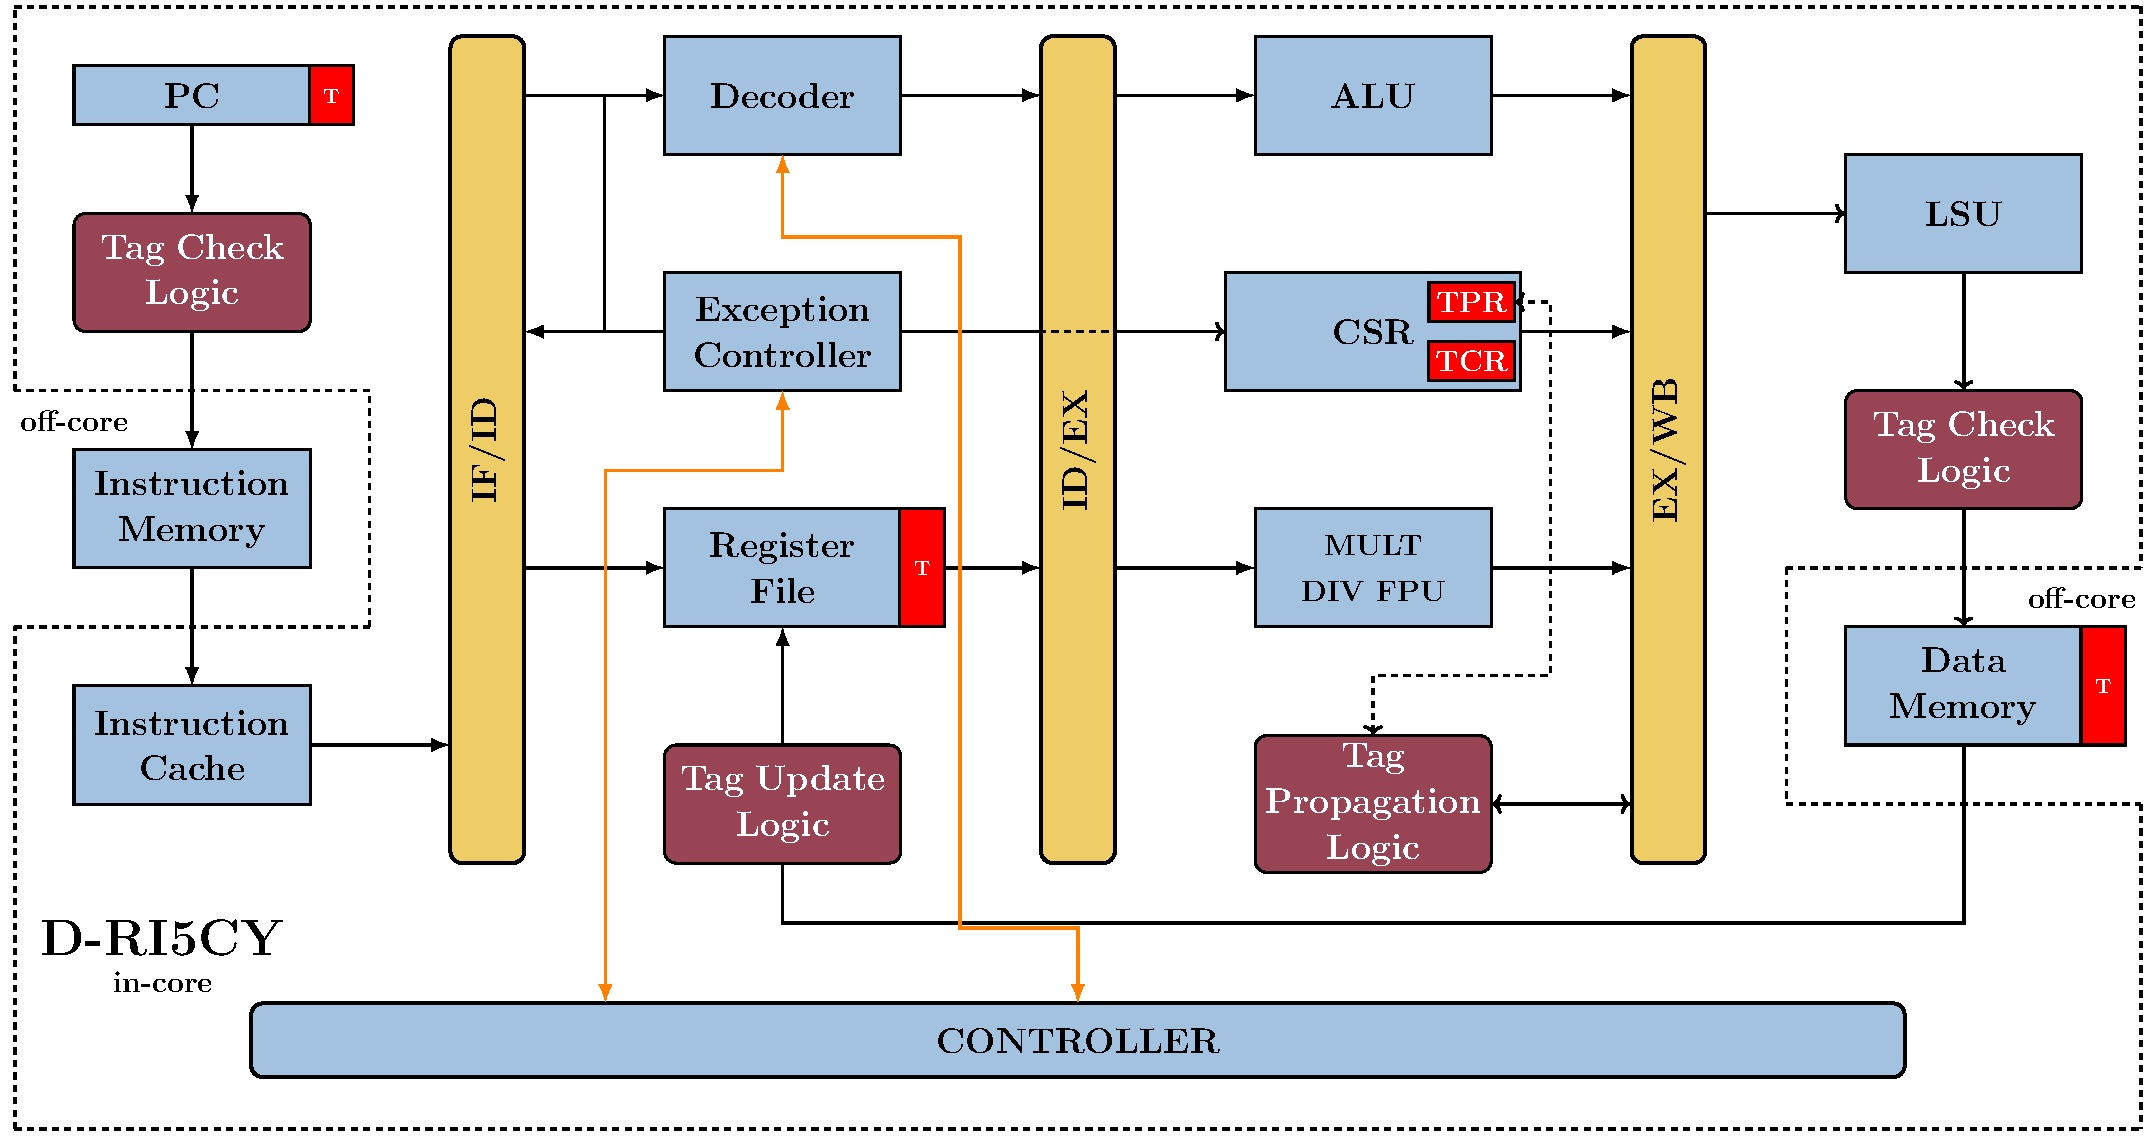
\includegraphics[width=.9\textwidth]{src/2_vuln_assessment/img/RI5CY.pdf}
        \caption{Architecture of the D-RI5CY.}
        \label{fig:riscy}
    \end{figure}
\end{frame}
%%%%%%%%%%%%%%%%%%%%%%%%%%%%%%%%%%%%%%%%%%%%%%%%%%%%%%%%%%%%%%%%%%%%%%%%%%%%
\subsection{Vulnerability assessment}
\begin{frame}{Vulnerability Assessment - Why?}
    \begin{block}{}
        We do a vulnerability assessment to:
        \begin{itemize}
            \setbeamertemplate{itemize items}[triangle]
            \justifying
            \item check if this DIFT is vulnerable against FIA,
            \item determine the spatial and temporal locations of vulnerabilities.
        \end{itemize}
    \end{block}
\end{frame}

\begin{frame}{Vulnerability Assessment - Threat model}
    \begin{block}{Threat model}
        We consider an attacker able to:
        \begin{itemize}
            \item perform a physical attack to defeat the DIFT mechanism and realise a software attack,
            \item inject faults in DIFT-related registers:
                  \begin{itemize}
                      \item bit set,
                      \item bit reset,
                      \item bit-flip.
                  \end{itemize}
        \end{itemize}
    \end{block}

    \begin{block}{Methodology}
        \begin{itemize}
            \item Analysis of 3 use cases: buffer overflow attack, format string attack, and compare/compute
            \item We do a temporal, and logical analysis of the tag propagation
        \end{itemize}
    \end{block}
\end{frame}
%%%%%%%%%%%%%%%%%%%%%%%%%%%%%%%%%%%%%%%%%%%%%%%%%%%%%%%%%%%%%%%%%%%%%%%%%%%%
\subsection{Use case : presentation}
\begin{frame}{Case: Buffer overflow}
    \begin{itemize}
        \item The attacker exploits a buffer overflow to access the return address register ($RA$).
    \end{itemize}

    \begin{figure}
        \centering
        \begin{subfigure}[l]{.45\textwidth}
            \centering
            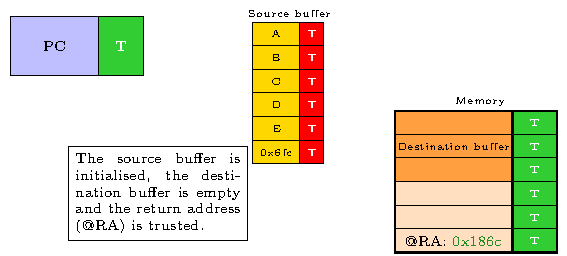
\includegraphics[width=.9\textwidth, page=1]{src/2_vuln_assessment/img/buffer_overflow/schemaPedagogique.pdf}
            \caption{Initialisation}
            \label{fig:bo_1st_step}
        \end{subfigure}
        \begin{subfigure}[r]{.45\textwidth}
            \centering
            \includegraphics[width=.9\textwidth, page=2]{src/2_vuln_assessment/img/buffer_overflow/schemaPedagogique.pdf}
            \caption{Copy of the source buffer into the destination buffer}
            \label{fig:bo_2_step}
        \end{subfigure}
    \end{figure}

    \begin{itemize}
        \item As the data in the source buffer is manipulated by the user, it is marked as \textcolor{red}{\textit{untrusted}}.
        \item Thanks to the DIFT, the tags associated with the source buffer data overwrite the memory tags.
    \end{itemize}
\end{frame}

\begin{frame}{Case: Buffer overflow}
    \begin{figure}
        \centering
        \begin{subfigure}[l]{.45\textwidth}
            \centering
            \includegraphics[width=.9\textwidth, page=3]{src/2_vuln_assessment/img/buffer_overflow/schemaPedagogique.pdf}
            \caption{An overflow occurs, the $RA$ register is overwritten}
            \label{fig:bo_3_step}
        \end{subfigure}
        \begin{subfigure}[r]{.45\textwidth}
            \centering
            \includegraphics[width=.9\textwidth, page=4]{src/2_vuln_assessment/img/buffer_overflow/schemaPedagogique.pdf}
            \caption{Corrupted $RA$ register is loaded into the PC}
            \label{fig:bo_4_step}
        \end{subfigure}
    \end{figure}

    \begin{itemize}
        \item Thanks to the DIFT, the tags associated with the source buffer data overwrite the $RA$ register tag.
        \item When the function ends, the corrupted register $RA$ is loaded into $PC$ using a jalr instruction.
    \end{itemize}
\end{frame}

\begin{frame}{Case: Buffer overflow}
    \begin{figure}
        \centering
        \includegraphics[width=.5\textwidth, page=5]{src/2_vuln_assessment/img/buffer_overflow/schemaPedagogique.pdf}
        \caption{PC address instruction is fetched}
        \label{fig:bo_5th_step}
    \end{figure}

    \begin{itemize}
        \item The $PC$ has been overwritten, it is now \textcolor{red}{untrusted}.
        \item The $PC$ address is fetched to access the next address.
    \end{itemize}
\end{frame}

\begin{frame}{Temporal analysis of the tag propagation}
    \begin{figure}
        \centering
        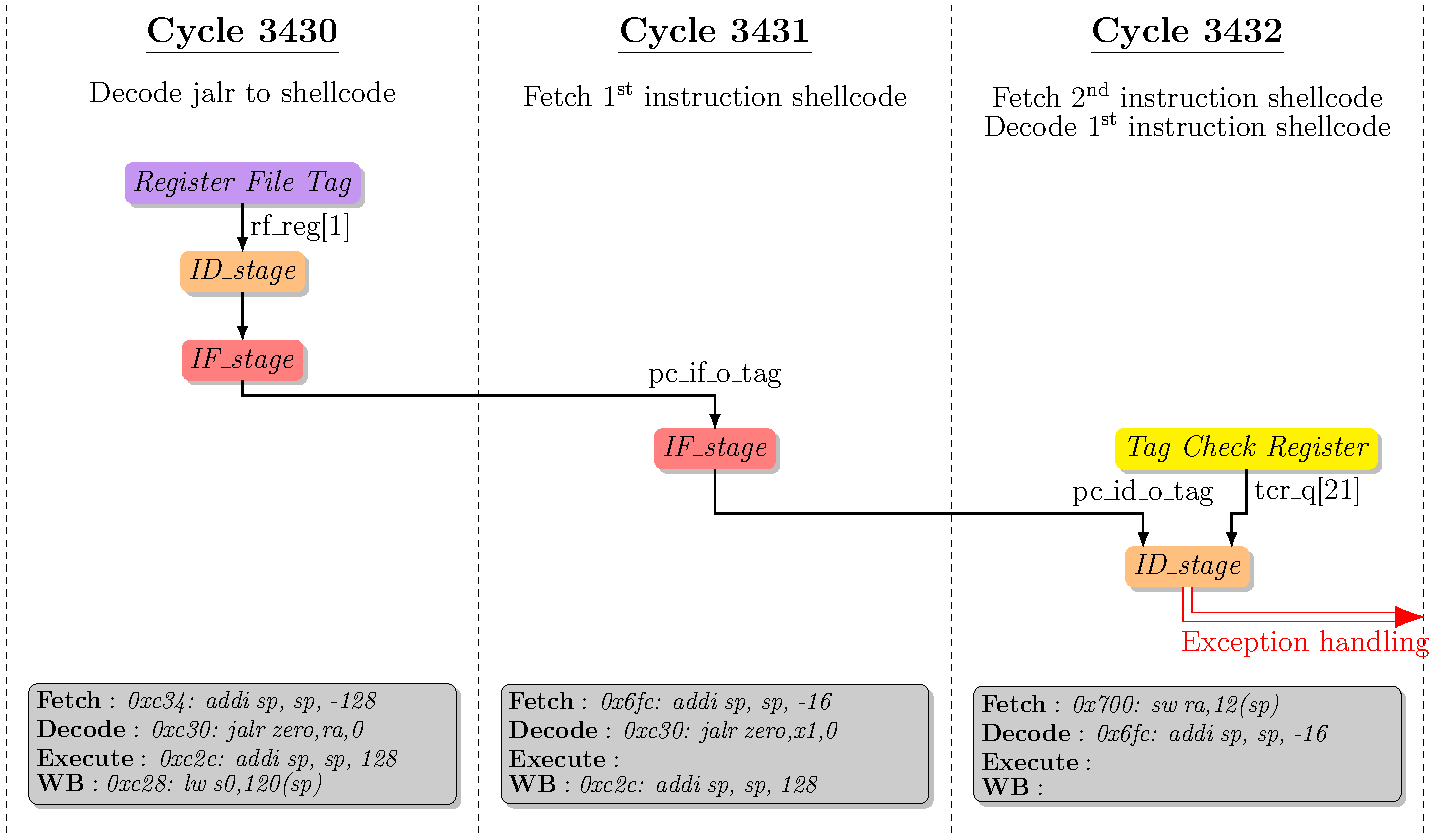
\includegraphics[width=.75\textwidth]{src/2_vuln_assessment/img/buffer_overflow/bufferOverflowAttack_short.pdf}
        \caption{Temporal analysis of tags propagation in a \textit{Buffer Overflow} attack}
        \label{fig:analyseTempoBufferOverflow}
    \end{figure}
\end{frame}

\begin{frame}{Logical analysis of the tag propagation}
    \begin{figure}
        \centering
        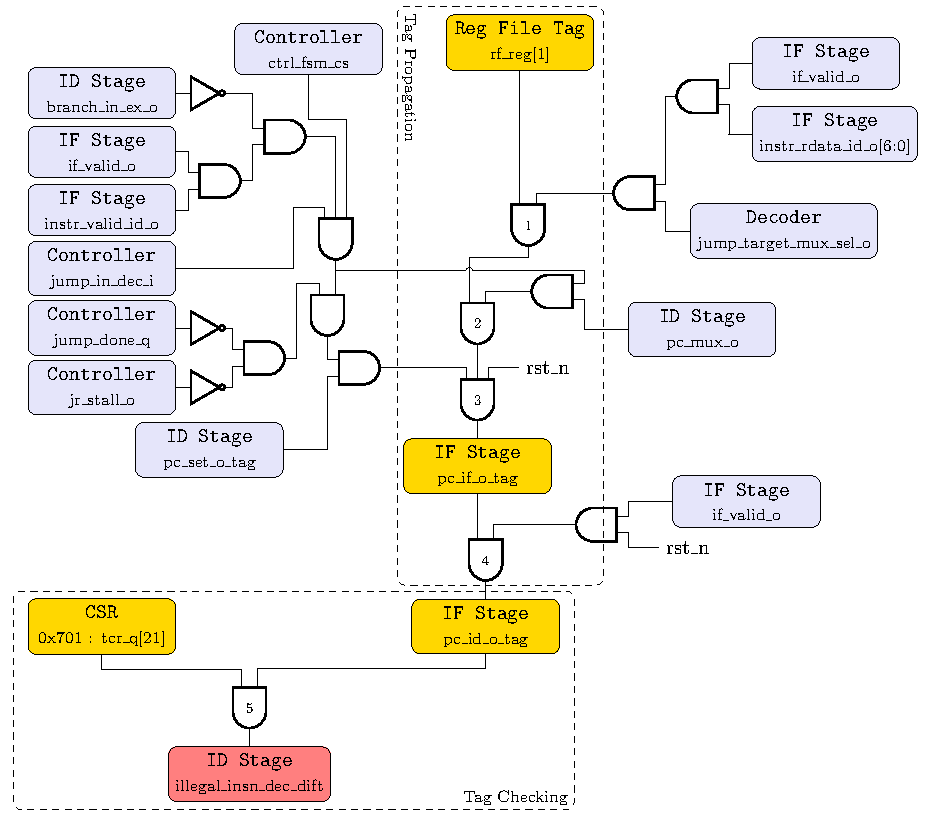
\includegraphics[height=.85\textheight]{src/2_vuln_assessment/img/buffer_overflow/arborescence_bufferOverflow.pdf}
        \caption{Logical analysis of tags propagation in a \textit{Buffer Overflow} attack}
        \label{fig:analyseLogiqueBufferOverflow}
    \end{figure}
\end{frame}
%%%%%%%%%%%%%%%%%%%%%%%%%%%%%%%%%%%%%%%%%%%%%%%%%%%%%%%%%%%%%%%%%%%%%%%%%%%%%%%%%%%%%%%%%%%%%%%%%%%%%%%%%%%%
\subsection{Experimental Setup}
%%%%%%%%%%%%%%%%%%%%%%%%%%%%%%%%%%%%%%%%%%%%%%%%%%%%%%%%%%%%%%%%%%%%%%%%%%%%%%%%%%%%%%%%%%%%%%%%%%%%%%%%%%%%
\begin{frame}{Experimental Setup - Simulation fault injections campaign}
    \begin{columns}
        \begin{column}{.125\linewidth}
            \hfill
        \end{column}
        \begin{column}{.75\linewidth}
            \begin{itemize}
                \justifying
                \item Logical fault injection simulation is used for preliminary evaluations
                      \begin{itemize}
                          \justifying
                          \item faults are injected in the HDL code at cycle accurate and bit accurate level
                          \item a set of 55 DIFT-related registers are targeted
                          \item a reference simulation is done without fault
                          \item results are classed in four groups
                                \begin{itemize}
                                    \justifying
                                    \item crash: reference cycle count exceeded,
                                    \item silent: current faulted simulation is the same as the reference simulation
                                    \item delay: illegal instruction is delayed
                                    \item success: DIFT has been bypassed
                                \end{itemize}
                      \end{itemize}
                \item Simulations with QuestaSim 10.6e.
                \item FISSA (presented later) is used in order to create our injection campaigns
            \end{itemize}
        \end{column}
        \begin{column}{.125\linewidth}
            \hfill
        \end{column}
    \end{columns}
\end{frame}
%%%%%%%%%%%%%%%%%%%%%%%%%%%%%%%%%%%%%%%%%%%%%%%%%%%%%%%%%%%%%%%%%%%%%%%%%%%%%%%%%%%%%%%%%%%%%%%%%%%%%%%%%%%%
\begin{frame}{Buffer overflow}
    \begin{table}
        \centering
        \small
        \caption{End of simulation status}
        \label{table:end_sim_by_status}
        \begin{tabular}{@{}rccccc@{}}
            \toprule
                            & Crash & NSTR & Delay & Success     & Total \\
            \midrule
            Buffer overflow & 0     & 1380 & 20    & 24 (1.69\%) & 1422  \\
            \bottomrule
        \end{tabular}
    \end{table}

    \begin{table}
        \centering
        \scriptsize
        \caption{Buffer overflow : Register sensitivity as determined by fault model and simulation time}
        \label{table:end_sim_from_time_fault_register_buffer_overflow}
        \setlength{\tabcolsep}{3pt}
        \begin{tabular}{@{}lccccccccccccccc@{}}
            \toprule
                                            & \multicolumn{3}{c}{Cycle 3428} & \multicolumn{3}{c}{Cycle 3429} & \multicolumn{3}{c}{Cycle 3430} & \multicolumn{3}{c}{Cycle 3431} & \multicolumn{3}{c}{Cycle 3432}                                                                                                                                                                                                                                            \\\cmidrule(lr){2-4}\cmidrule(lr){5-7}\cmidrule(lr){8-10}\cmidrule(lr){11-13}\cmidrule(lr){14-16}
                                            & set0                           & set1                           & bitflip                        & set0                           & set1                           & bitflip                      & set0                        & set1 & bitflip                      & set0                        & set1 & bitflip                      & set0                        & set1 & bitflip                      \\
            \midrule
            pc\_if\_o\_tag                  &                                &                                &                                &                                &                                &                              &                             &      &                              & \textcolor{red}{\checkmark} &      & \textcolor{blue}{\checkmark} &                             &      &                              \\
            memory\_set\_o\_tag             &                                & \textcolor{LimeGreen}{\checkmark}  & \textcolor{blue}{\checkmark}   &                                &                                &                              &                             &      &                              &                             &      &                              &                             &      &                              \\
            rf\_reg[1]                      &                                &                                &                                &                                &                                &                              & \textcolor{red}{\checkmark} &      & \textcolor{blue}{\checkmark} &                             &      &                              &                             &      &                              \\
            tcr\_q                          & \textcolor{red}{\checkmark}    &                                &                                & \textcolor{red}{\checkmark}    &                                &                              & \textcolor{red}{\checkmark} &      &                              & \textcolor{red}{\checkmark} &      &                              & \textcolor{red}{\checkmark} &      &                              \\
            \rowcolor{LightGray} tcr\_q[21] &                                &                                & \textcolor{blue}{\checkmark}   &                                &                                & \textcolor{blue}{\checkmark} &                             &      & \textcolor{blue}{\checkmark} &                             &      & \textcolor{blue}{\checkmark} &                             &      & \textcolor{blue}{\checkmark} \\
            tpr\_q                          & \textcolor{red}{\checkmark}    & \textcolor{LimeGreen}{\checkmark}  &                                & \textcolor{red}{\checkmark}    & \textcolor{LimeGreen}{\checkmark}  &                              &                             &      &                              &                             &      &                              &                             &      &                              \\
            \rowcolor{LightGray} tpr\_q[12] &                                &                                & \textcolor{blue}{\checkmark}   &                                &                                & \textcolor{blue}{\checkmark} &                             &      &                              &                             &      &                              &                             &      &                              \\
            \rowcolor{LightGray} tpr\_q[15] &                                &                                & \textcolor{blue}{\checkmark}   &                                &                                & \textcolor{blue}{\checkmark} &                             &      &                              &                             &      &                              &                             &      &                              \\
            \bottomrule
        \end{tabular}
    \end{table}
\end{frame}

\begin{frame}{Summary}
    \begin{columns}
        \begin{column}{.15\linewidth}
            \hfill
        \end{column}
        \begin{column}{.7\linewidth}
            \begin{itemize}
                \setbeamertemplate{itemize items}[triangle]
                \item 4266 simulations have been performed,
                \item 95 successes (2.23\%).
                \item This campaign showed 43 highly sensitive registers on 55 DIFT-related registers
                \item We have shown that the D-RI5CY DIFT is vulnerable to FIA
                \item Propagation of faults is facilitated by paths fully made of \textit{AND} gates
            \end{itemize}

            % \begin{block}{}
                \begin{itemize}
                    \setbeamertemplate{itemize items}[triangle]
                    \item Best paper at Sensors S\&P 2023~\cite{PLG-23-SensorsSP}.
                \end{itemize}
            % \end{block}
        \end{column}
        \begin{column}{.15\linewidth}
            \hfill
        \end{column}
    \end{columns}
    
\end{frame}
%%%%%%%%%%%%%%%%%%%%%%%%%%%%%%%%%%%%%%%%%%%%%%%%%%%%%%%%%%%%%%%%%%%%%%%%%%%%%%%%%%%%%%%%%%%%%%%%%%%%%%%%%%%%